\section{Exercise 03: General Assessment}
\subsection{Finding information with whois}


\subsubsection{What do you learn about SDUs network? In the protocol, note the IPrange.}

\begin{figure}[H]
    \centering
    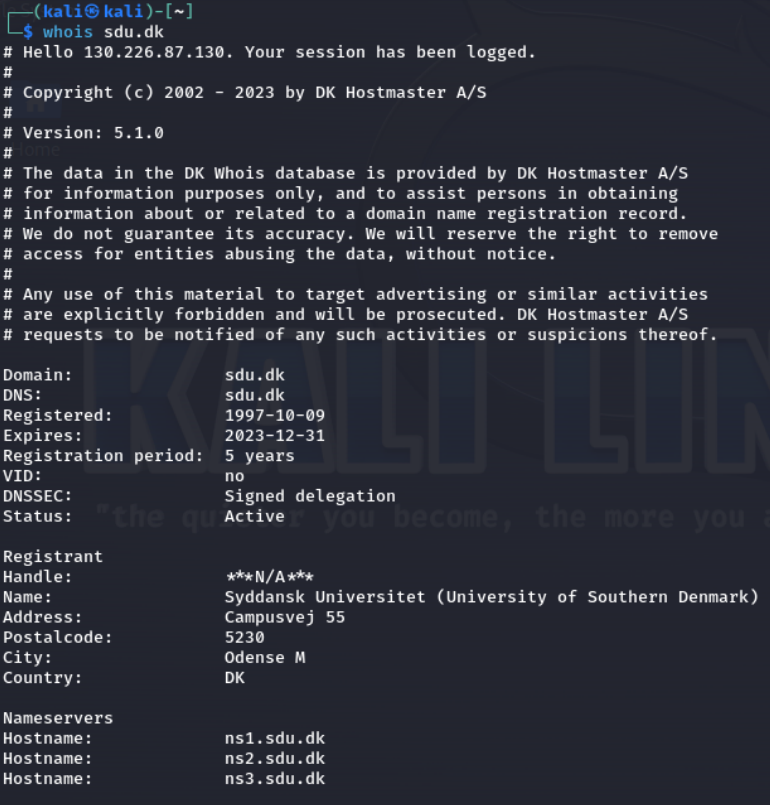
\includegraphics[width=0.8\linewidth]{pic/whois SDU 1.png}
    \caption{whois SDU 1}
    \label{fig:whois SDU 1}
\end{figure}

\begin{figure}[H]
    \centering
    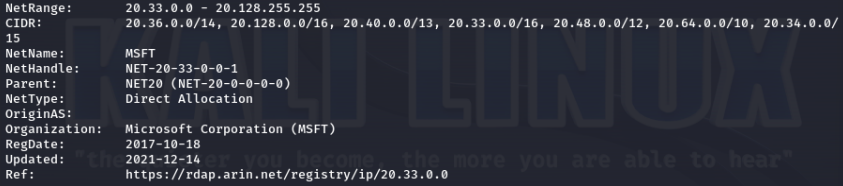
\includegraphics[width=0.8\linewidth]{pic/whois SDU 2.png}
    \caption{whois SDU 2}
    \label{fig:whois SDU 2}
\end{figure}

\textbf{www.sdu.dk} (IP: 20.105.224.27)
\begin{itemize}
    \item This IP address is a part of the 20.33.0.0 - 20.128.255.255 IP range.
    \item It is registered under the Microsoft Corporation (MSFT) and is a part of the Microsoft Azure cloud platform.
    \item The organization's address is One Microsoft Way, Redmond, WA, 98052, US.
\end{itemize}

The CIDR which is also given are:
\begin{itemize}
    \item 20.33.0.0/14
    \item 20.128.0.0/16
    \item 20.40.0.0/13
    \item 20.33.0.0/16
    \item 20.48.0.0/12
    \item 20.64.0.0/10
    \item 20.34.0.0/15
\end{itemize}




\subsubsection{What is the whois information for nextcloud.sdu.dk ? What do you observe in comparison to the whois-information you gathered for www.sdu.dk.}

\begin{figure}[H]
    \centering
    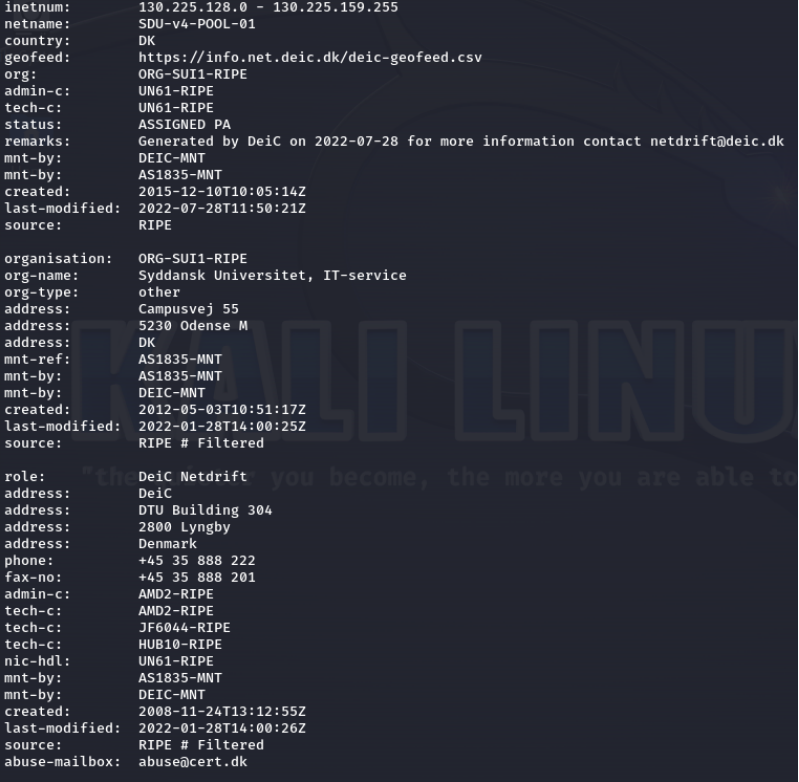
\includegraphics[width=\linewidth]{pic/nextcloud 1.png}
    \caption{nextcloud 1}
    \label{fig:nextcloud 1}
\end{figure}

\begin{figure}[H]
    \centering
    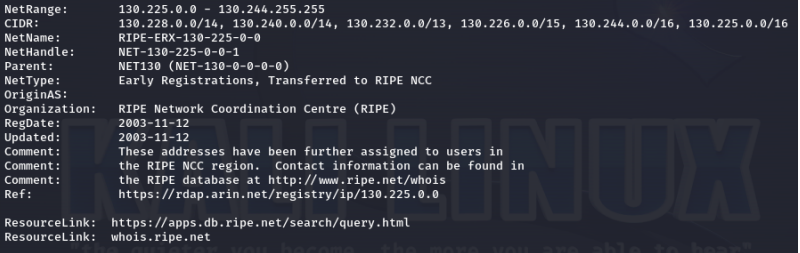
\includegraphics[width=\linewidth]{pic/nextcloud 2.png}
    \caption{nextcloud 2}
    \label{fig:nextcloud 2}
\end{figure}

\textbf{nextcloud.sdu.dk} (IP: 130.225.156.61)
\begin{itemize}
    \item This IP address falls within the range of 130.225.0.0 - 130.244.255.255.
    \item It is associated with the RIPE Network Coordination Centre which generally covers European regions.
    \item Further details from the RIPE database show that this IP address range is specifically associated with Syddansk Universitet, IT-service. The address is Campusvej 55, 5230 Odense M, DK (Denmark).
\end{itemize}

\textbf{Comparison}

The result given from \textit{nextcloud.sdu.dk} looks alot like the outcome of querying the IP address \textit{sdu.dk}.
The IP range for "nextcloud.sdu.dk" differs, spanning from 130.225.128.0 to 130.225.159.255.


\subsection{Question: nmap}
To configure Nmap scans for sending packets with specific IP options and for MAC address spoofing, you would utilize the following.

\subsubsection{Send packets with specified ip options}
For setting specific IP options in the packets you send, the \textit{--ip-options} is used. This allows you to include various IP options required for the scan.

\subsubsection{Spoof your MAC address}
To spoof your MAC address, the \textit{--spoof-mac} option is employed. This can be used to input a particular MAC address or to instruct Nmap to generate a random one for the scan.




\subsection{Comparing the Tools}
\subsubsection{Compare your results from each of the previous activities in each question (e.g., sparta vs nessus vs openvas). Take notes \& discuss overlaps and differences inresults, pros and cons, ease of use for each tool.}

\subsection*{Overlaps}
\begin{itemize}
    \item All tools serve the purpose of vulnerability assessment.
    \item They can identify common vulnerabilities and security flaws.
    \item Network scanning capabilities are present in all three.
\end{itemize}

\subsection*{Differences}
\begin{itemize}
    \item Legion is open-source with a focus on network penetration and requires higher technical literacy.
    \item Nessus is closed-source, designed for user-friendliness, and oriented towards scanning efficiency.
    \item GVM is open-source with an emphasis on customization for power users.
\end{itemize}

\subsection*{Pros and Cons}
\subsubsection*{Legion}
\textbf{Pros:}
\begin{itemize}
    \item Open-source nature permits custom scripting.
\end{itemize}
\textbf{Cons:}
\begin{itemize}
    \item Less user-friendly and demands technical knowledge.
\end{itemize}

\subsubsection*{Nessus}
\textbf{Pros:}
\begin{itemize}
    \item Highly user-friendly interface.
\end{itemize}
\textbf{Cons:}
\begin{itemize}
    \item Commercial product and less customizable.
\end{itemize}

\subsubsection*{GVM}
\textbf{Pros:}
\begin{itemize}
    \item Open-source with a frequently updated vulnerability database and high customizability.
\end{itemize}
\textbf{Cons:}
\begin{itemize}
    \item Not as intuitive for novices compared to Nessus.
\end{itemize}

\subsection*{Ease of Use}
\begin{itemize}
    \item \textit{Legion}: Offers a technical interface suited for experienced users.
    \item \textit{Nessus}: Focuses on ease of use with a user-friendly design.
    \item \textit{GVM}: Presents a complex interface, beneficial for advanced users who seek customization.
\end{itemize}







\subsection{Collecting the Assessment Information}
Stared by doing \textit{nmap -sn 10.0.2.0/24} with the result below.

\begin{figure}[H]
    \centering
    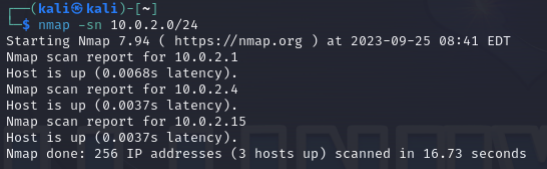
\includegraphics[width=0.7\linewidth]{pic/nmap sn.png}
    \caption{\textit{nmap -sn 10.0.2.0/24}}
    \label{fig:nmap sn}
\end{figure}

Then scanned the ports \textit{10.0.2.1, 10.0.2.4} and \textit{10.0.2.15}
With the result below from the \textit{10.0.2.15} scan.

\begin{figure}[H]
    \centering
    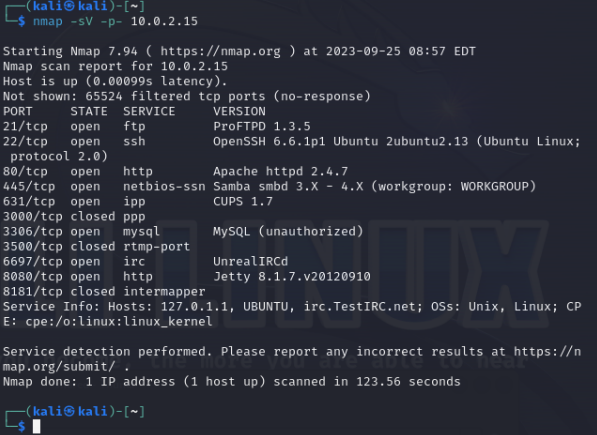
\includegraphics[width=0.7\linewidth]{pic/nmap sv.png}
    \caption{\textit{nmap -sv -p- 10.0.2.15}}
    \label{fig:nmap sv}
\end{figure}

\subsubsection{Service, port number and version number, e.g., FTP 21 vxxxx}
Based on the ablow scans the following 4 services, ports, states, services, and verions were found and analyzed below.

\begin{itemize}
    \item \textbf{Service:} FTP, Port: 21, Version: ProFTPD 1.3.5
          \begin{itemize}
              \item \textbf{Vulnerability:} ProFTPD has a critical flaw that permits unauthenticated file copying, potentially leading to remote code execution.
              \item \textbf{Severity:} Extremely high, as remote code execution can have devastating consequences on system integrity.
              \item \textbf{Source:} CVE-2015-3306
          \end{itemize}

    \item \textbf{Service:} SSH, Port: 22, Version: OpenSSH 6.6.1p1 Ubuntu 2ubuntu2.13
          \begin{itemize}
              \item \textbf{Vulnerability:} OpenSSH has a vulnerability that allows login into a minikube container using default credentials, essentially sidestepping authentication measures.
              \item \textbf{Severity:} Very high, as it compromises SSH security potentially giving complete unauthorized shell access.
              \item \textbf{Source:} CVE-2023-1944
          \end{itemize}

    \item \textbf{Service:} HTTP, Port: 80, Version: Apache httpd 2.4.7
          \begin{itemize}
              \item \textbf{Vulnerability:} The Drupal coder module accessible via Apache’s open directory listing permits remote code execution.
              \item \textbf{Severity:} Very high, as it could allow an attacker to run arbitrary code on the server.
              \item \textbf{Source:} https://www.drupal.org/node/2765575
          \end{itemize}

    \item \textbf{Service:} IPP, Port: 631, Version: CUPS 1.7
          \begin{itemize}
              \item \textbf{Vulnerability:} Utilizes outdated TLS versions, which could be exploited to decrypt traffic, risking the confidentiality of transmitted data.
              \item \textbf{Severity:} Moderate, depending on whether sensitive data is being transmitted.
              \item \textbf{Source:} CVE-2011-3389
          \end{itemize}
\end{itemize}



\subsection{Completing the Assessment - Final report}

\textbf{Security Synopsis:}
The assessment indicates that the Linux platform contains several critical vulnerabilities, with remote code execution and reverse shell capabilities among them.
These issues are severe and could result in full system compromise.

\textbf{Prioritization and Remediation Strategy:}
\begin{itemize}
    \item Immediate Action: Services with the potential for remote code execution, like FTP running ProFTPD 1.3.5, are to be prioritized for urgent patching due to their high criticality.
    \item Regular Updates: Following immediate mitigation, a regime of regular updates and patches is crucial to maintain a secure state.
    \item Ongoing Vigilance: Tools such as GVM should be employed for continuous monitoring and regular security assessments to identify and patch any new vulnerabilities promptly.
\end{itemize}

\textbf{Critical Vulnerabilities:}
\begin{itemize}
    \item \textit{FTP - ProFTPD 1.3.5 (CVE-2015-3306)}: High risk due to the possibility of unauthorized access and control over the system.
\end{itemize}

\textbf{Recommendations:}
\begin{itemize}
    \item Systems exhibiting critical vulnerabilities should be taken offline and updated to secure versions before being reinstated.
    \item Implement continuous monitoring systems to detect and rectify new vulnerabilities.
    \item Conduct regular security training for employees to mitigate risks from social engineering attacks.
    \item Perform systematic security audits to stay ahead of potential security threats.
\end{itemize}




